\documentclass[
  %ignorenonframetext,
  aspectratio=1610,
]{beamer}

\usepackage{Helmholtz-AI}
%% extrapackages added from markdown frontmatter
\usepackage{fontawesome5}
\usepackage{xspace} 
\usepackage{lmodern}
\usepackage{graphicx}
\usepackage{booktabs}
\usepackage{tabularx}
\usepackage{array}
\usepackage{xspace}
\usepackage{verbatim}
\usepackage{listings}
\usepackage{pifont}
\usepackage{ulem}
\usepackage{media9}
\usepackage{enumitem}
% References
% \usepackage[
%   backend=biber,
%   url=true,
%   sorting=none,
%   ]{biblatex}
%   \addbibresource{references.bib}
\usepackage{hyperref}

\definecolor{applegreen}{rgb}{0.55, 0.71, 0.0}
\definecolor{cadmiumred}{rgb}{0.89, 0.0, 0.13}
  
\providecommand{\tightlist}{%
  \setlength{\itemsep}{0pt}\setlength{\parskip}{0pt}}

% add labels to itemize
\setlist[itemize,1]{label=\textbullet}
\setlist[itemize,2]{label=\textopenbullet}

\hypersetup{
  colorlinks=true,
  linkcolor=hgfblue,
  filecolor=Maroon,
  citecolor=hgfinformation,
  urlcolor=hgfmatter,
  pdfcreator={Till Korten}
  }

\usepackage{tikz}
\usetikzlibrary{positioning}
\usetikzlibrary{arrows.meta}

% LISTINGS SETUP (for code)
\lstdefinestyle{code}{
basicstyle=\ttfamily\footnotesize,
keywordstyle=\bfseries,
commentstyle=\itshape,
showstringspaces=false,
columns=fullflexible,
frame=single,
breaklines=true,
tabsize=2
}

% SHORTCUTS
\newcommand{\cmark}{\ding{51}} % checkmark
\newcommand{\xmark}{\ding{55}} % xmark
\newcommand{\tool}[1]{\texttt{#1}}

\title{Abstracts Explorer: Navigating Conference Research with Agentic AI}
\subtitle{Helmholtz AI Conference 2026}
\author{Thomas Wachtler}
\date{Helmholtz AI Conference 2026}
\institute{Forschungszentrum Jülich}
\titlegraphic{}


% BEGIN DOCUMENT
\begin{document}

% 1 — TITLE
\maketitle

% 1b — HOOK
\begin{frame}{Navigate Conference Research with Agentic AI}
  \begin{alertblock}{Imagine this scenario}
    You open the conference programme.\\
    6000 abstracts. 10+ parallel tracks. You have a 6h flight to prepare.\\
    Where do \textit{you} start?
  \end{alertblock}
  \vspace{0.5em}
  \textbf{Traditional approach:} skim titles $\rightarrow$ miss half the relevant work\\[0.3em]
  \textbf{Abstracts Explorer:} let an AI agent do the heavy lifting --- \textit{with you in control}
\end{frame}

% 4 — DEMO: SEARCH
\begin{frame}{More Relevant Results With Semantic Search}
  \begin{columns}[T]
    \begin{column}{0.55\textwidth}
      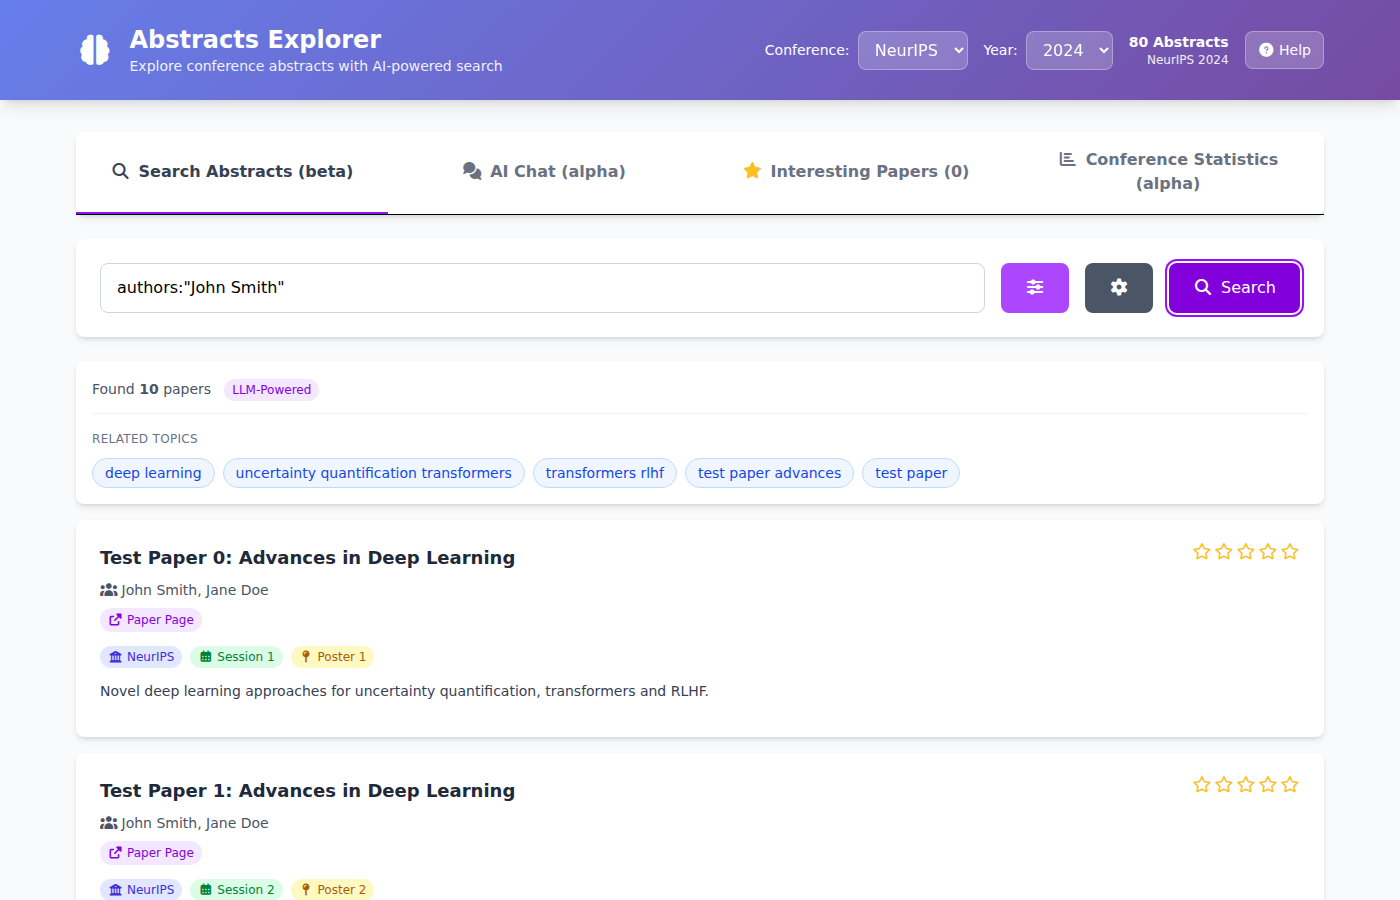
\includegraphics[width=\textwidth]{images/web-ui-search.png}
    \end{column}
    \begin{column}{0.42\textwidth}
      \begin{itemize}
        \item Semantic search (vector similarity) finds relevant abstracts based on meaning, not just keyword matches
        \item Filters: conference, year, track, decision type
        \item Results ranked by relevance
      \end{itemize}
    \end{column}
  \end{columns}
\end{frame}

% 5 — DEMO: CHAT
\begin{frame}{Chat With the Conference to Get an Overview}
  \begin{columns}[T]
    \begin{column}{0.45\textwidth}
      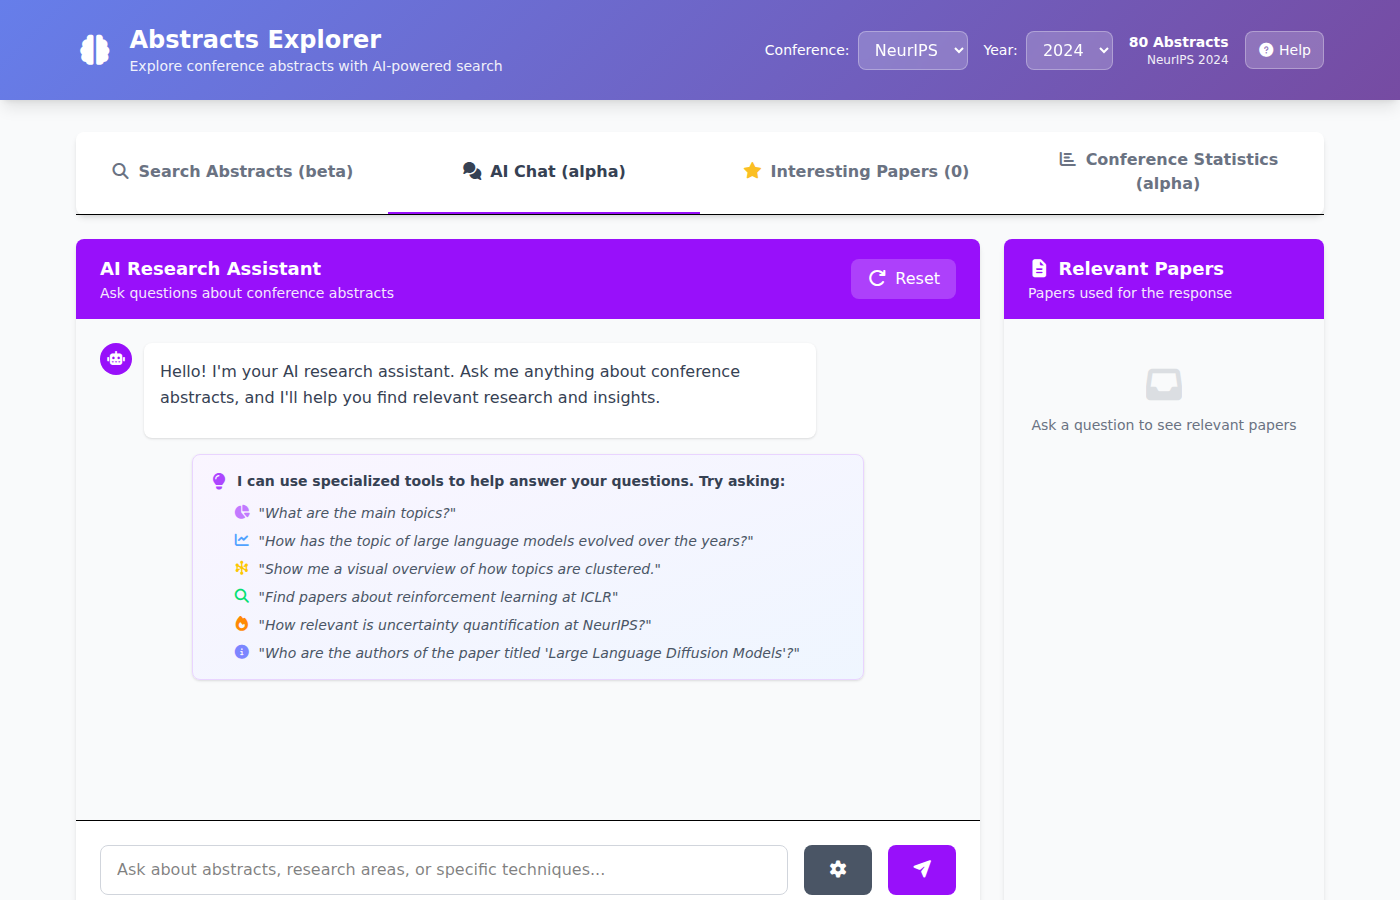
\includegraphics[width=\textwidth]{images/web-ui-chat.png}
    \end{column}
    \begin{column}{0.52\textwidth}
      \textbf{What happens under the hood:}
      \begin{enumerate}[label=\arabic*.]
        \item Query rewriting $\rightarrow$ clarify intent, expand acronyms
        \item Abstract retrieval $\rightarrow$ top-k from ChromaDB
        \item Context assembly $\rightarrow$ LLM reading list
        \item Tool invocation $\rightarrow$ MCP for trend/cluster analysis
        \item LLM response $\rightarrow$ grounded answer with citations and/or tool results
      \end{enumerate}
    \end{column}
  \end{columns}
\end{frame}

% 6a — DEMO: INTERESTING PAPERS
\begin{frame}{Rate Papers to Build Your Schedule}
  \begin{columns}[T]
    \begin{column}{0.55\textwidth}
      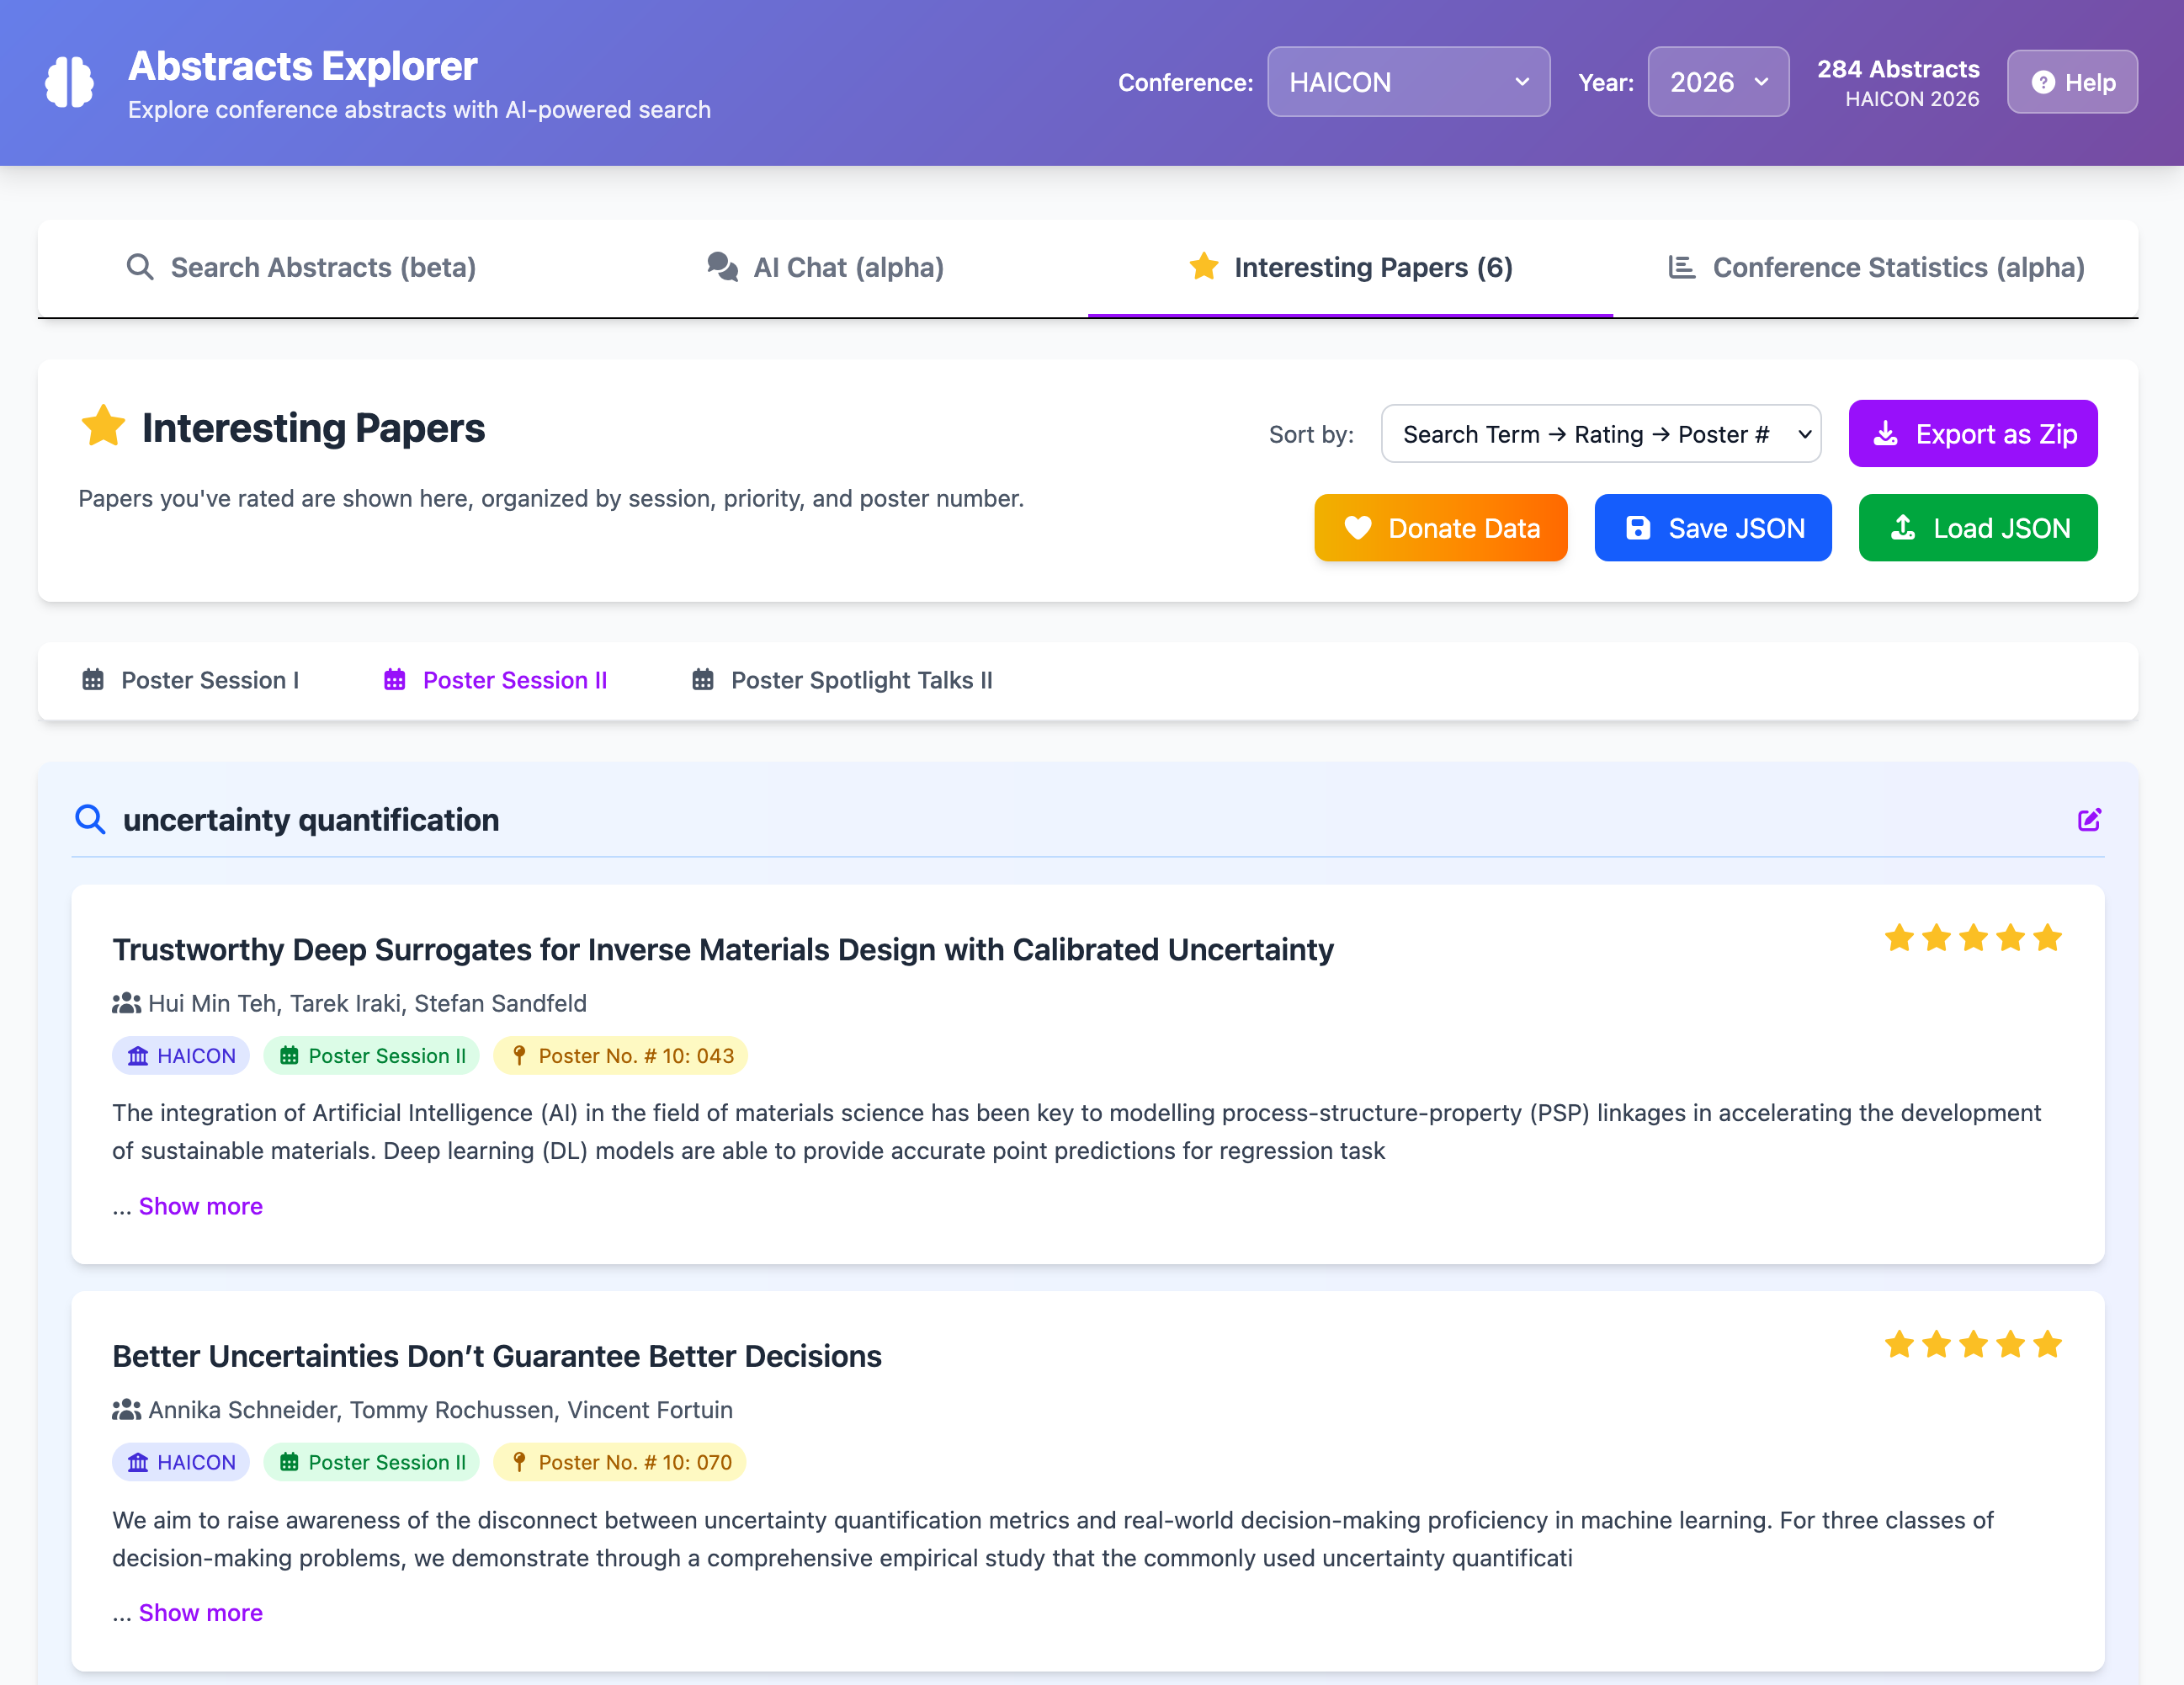
\includegraphics[width=\textwidth]{images/web-ui-interesting.png}
    \end{column}
    \begin{column}{0.45\textwidth}
      \textbf{Interesting Papers} (Tab~3)\\[0.5em]
      \begin{itemize}
        \item Rate abstracts 1--5 stars while browsing
        \item Export as ZIP / JSON / Markdown --- ready for your notes app
      \end{itemize}
    \end{column}
  \end{columns}
\end{frame}

% 6b — DEMO: STATS
\begin{frame}{Visualise the Topic Landscape}
  \begin{columns}[T]
    \begin{column}{0.33\textwidth}
      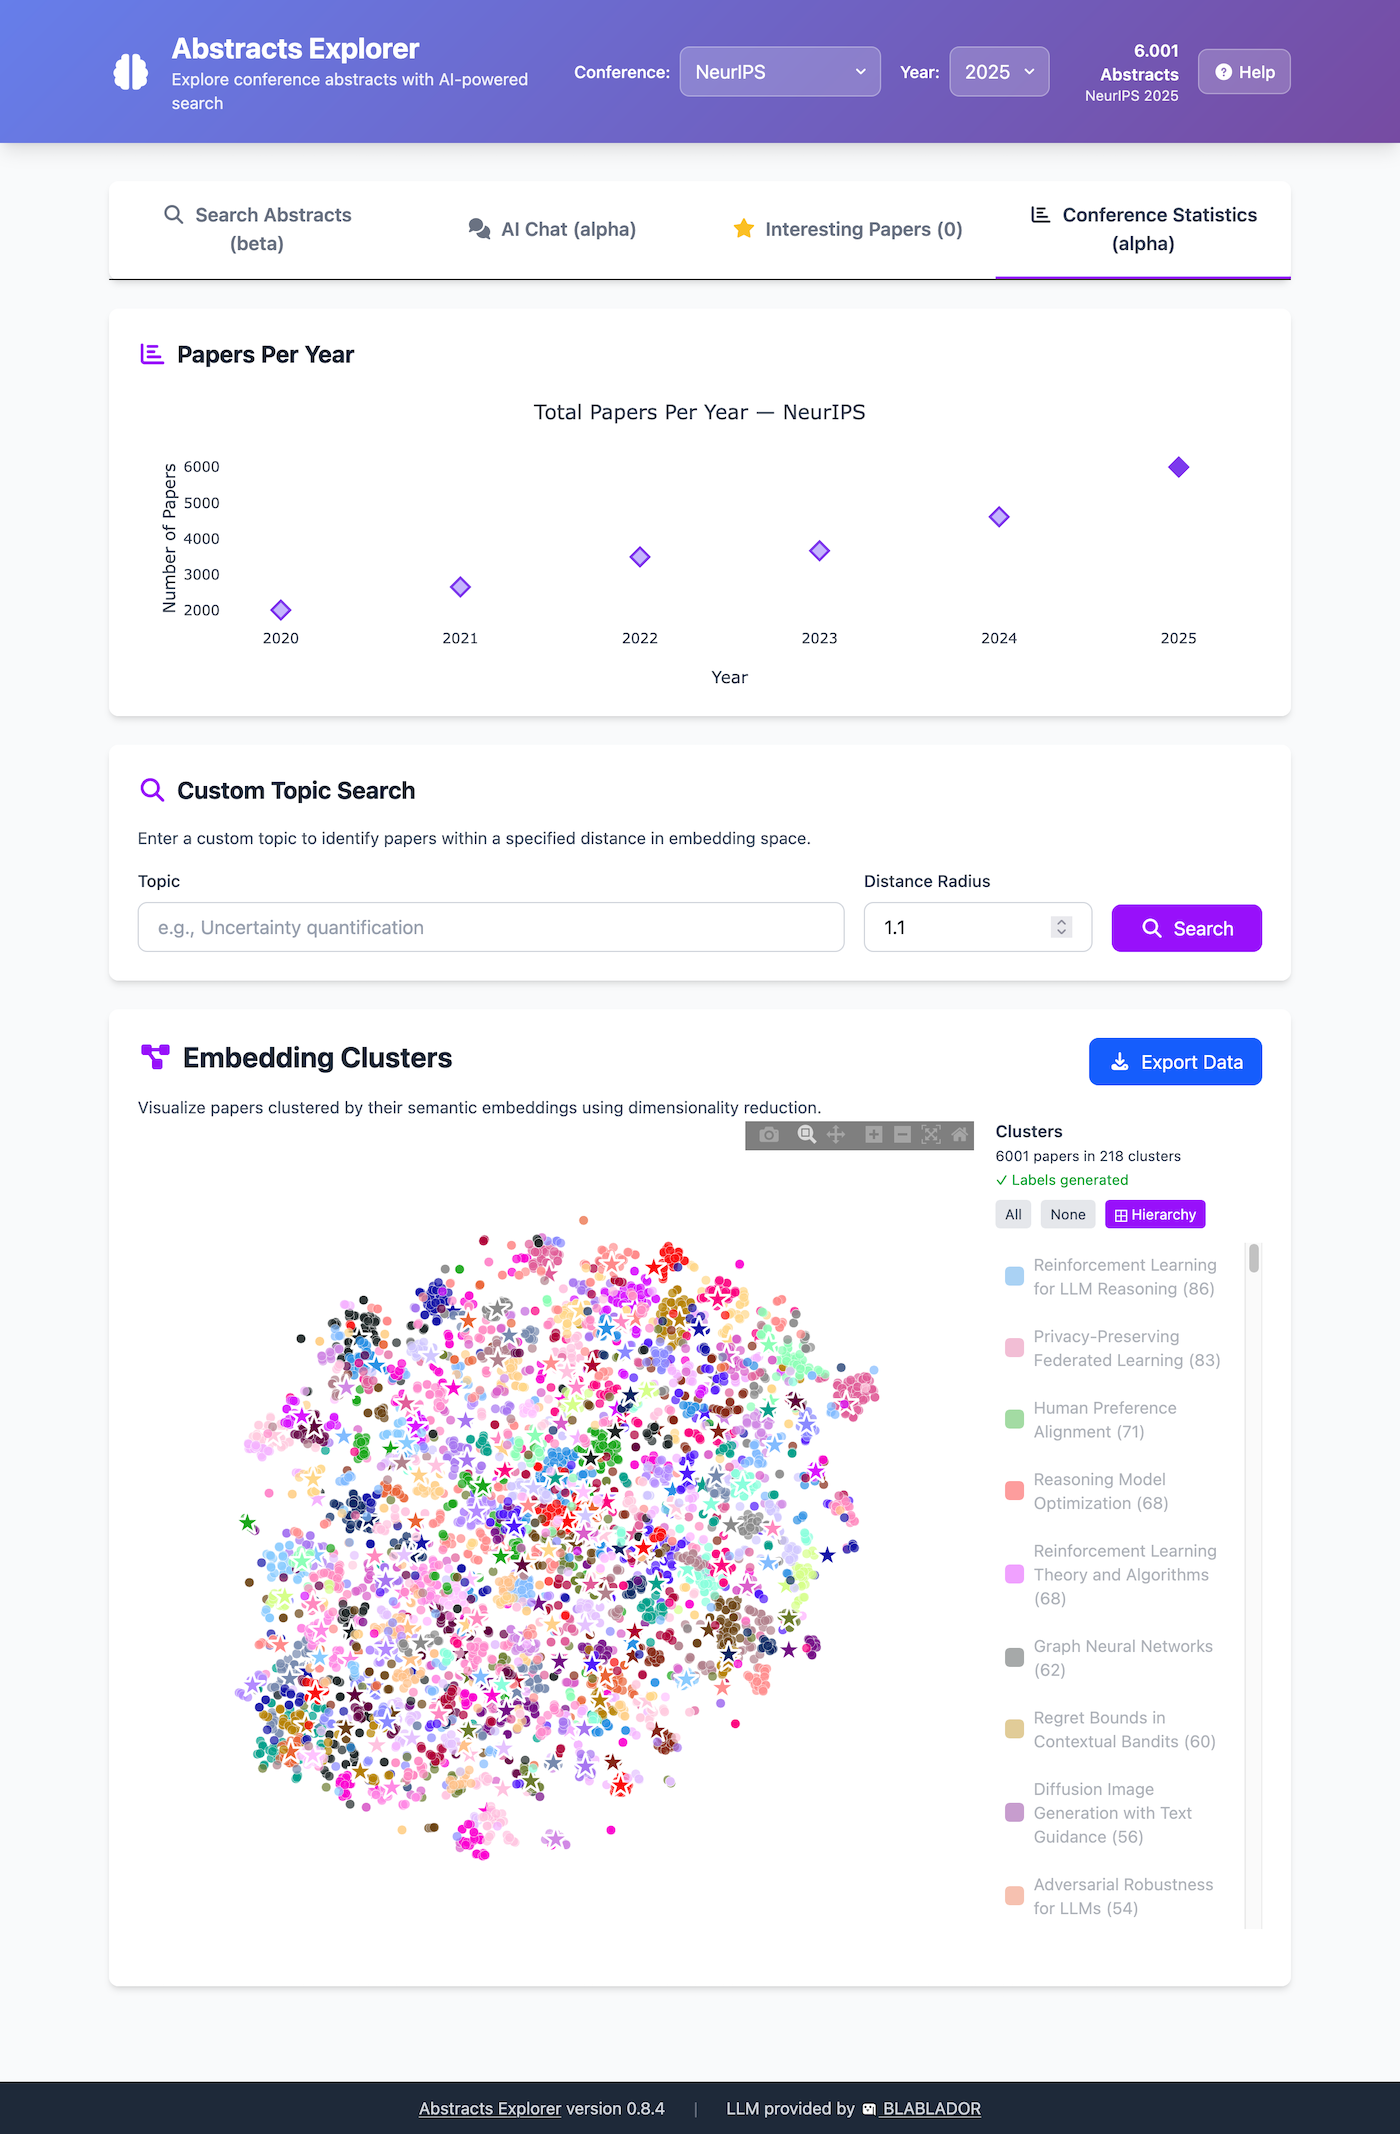
\includegraphics[width=\textwidth]{images/web-ui-statistics.png}
    \end{column}
    \begin{column}{0.66\textwidth}
      \textbf{Conference Statistics} (Tab~4)\\[0.5em]
      \begin{itemize}
        \item Topic trend chart
        \item Cluster landscape
        \item Agglomerative clustering of abstracts based on full embeddings (4k dimensions)
        \item t-sne dimensionality reduction for 2D visualisation
        \item LLM-generated cluster labels
        \item Basis for MCP tools:
              \begin{itemize}
                \item \texttt{get\_conference\_topics}
                \item \texttt{get\_cluster\_visualization}
                \item \texttt{analyze\_topic\_relevance}
                \item \texttt{get\_topic\_evolution}
              \end{itemize}
      \end{itemize}
    \end{column}
  \end{columns}
\end{frame}

\begin{frame}[fragile]{Agentic AI Definition}
  A system is \textbf{agentic} when it can:
  \begin{itemize}
    \item[1.] \textbf{Perceive} a goal expressed in natural language
    \item[2.] \textbf{Plan} which tools to invoke
    \item[3.] \textbf{Execute} those tools autonomously
    \item[4.] \textbf{Reflect} on results and loop back
  \end{itemize}
  \vspace{0.3em}
  \begin{verbatim}
User goal -> LLM planner -> tool calls -> results -> LLM answer
                 ^__________feedback loop__________^
  \end{verbatim}
\end{frame}

% DATA STACK
\begin{frame}{Abstracts Explorer Data Stack}
  \small
  \begin{tabularx}{\textwidth}{lX}
    \toprule
    \textbf{Layer}      & \textbf{What it does}                                     \\
    \midrule
    \textbf{Data}       & Downloads \& stores abstracts from 10+ conferences        \\
    \textbf{Embeddings} & Converts abstracts to vectors via an LLM embedding model  \\
    \textbf{Retrieval}  & Semantic (cosine similarity) search                       \\
    \textbf{Agency}     & MCP tools: the LLM decides which analysis to run          \\
    \textbf{Reasoning}  & RAG chat: the LLM answers questions based on tool results \\
    \textbf{Interface}  & Flask/Waitress web UI                                     \\
    \bottomrule
  \end{tabularx}
  \vspace{0.5em}
\end{frame}

\begin{frame}{MCP Gives the LLM a Toolbox to Choose From}
  \begin{block}{MCP: Model Context Protocol}
    MCP is an open standard for exposing \textbf{callable tools} to LLMs.
    The LLM reads the tool descriptions and decides \textit{when and how} to call them.
  \end{block}
  \vspace{0.3em}
  \textbf{The 6 MCP tools in Abstracts Explorer}\\[0.3em]
  \small
  \begin{tabularx}{\textwidth}{lX}
    \toprule
    \textbf{Tool}                      & \textbf{Question it answers}                             \\
    \midrule
    \tool{get\_conference\_topics}     & ``What are the main themes this year?''                  \\
    \tool{analyze\_topic\_relevance}   & ``How prominent is uncertainty quantification?''         \\
    \tool{get\_topic\_evolution}       & ``How has diffusion model research trended since 2020?'' \\
    \tool{search\_papers}              & ``Find papers about graph neural networks''              \\
    \tool{get\_cluster\_visualization} & ``Show me the topic landscape''                          \\
    \tool{get\_paper\_details}         & ``Who wrote that? Where is the poster?''                 \\
    \bottomrule
  \end{tabularx}
  \vspace{0.3em}
  \begin{block}{}
    No special syntax --- the LLM picks the right tool from your plain-English question.
  \end{block}
\end{frame}

% 8 — AGENTIC LOOP DIAGRAM
\begin{frame}{One Question Triggers a Chain of Tool Calls}
  \begin{center}
    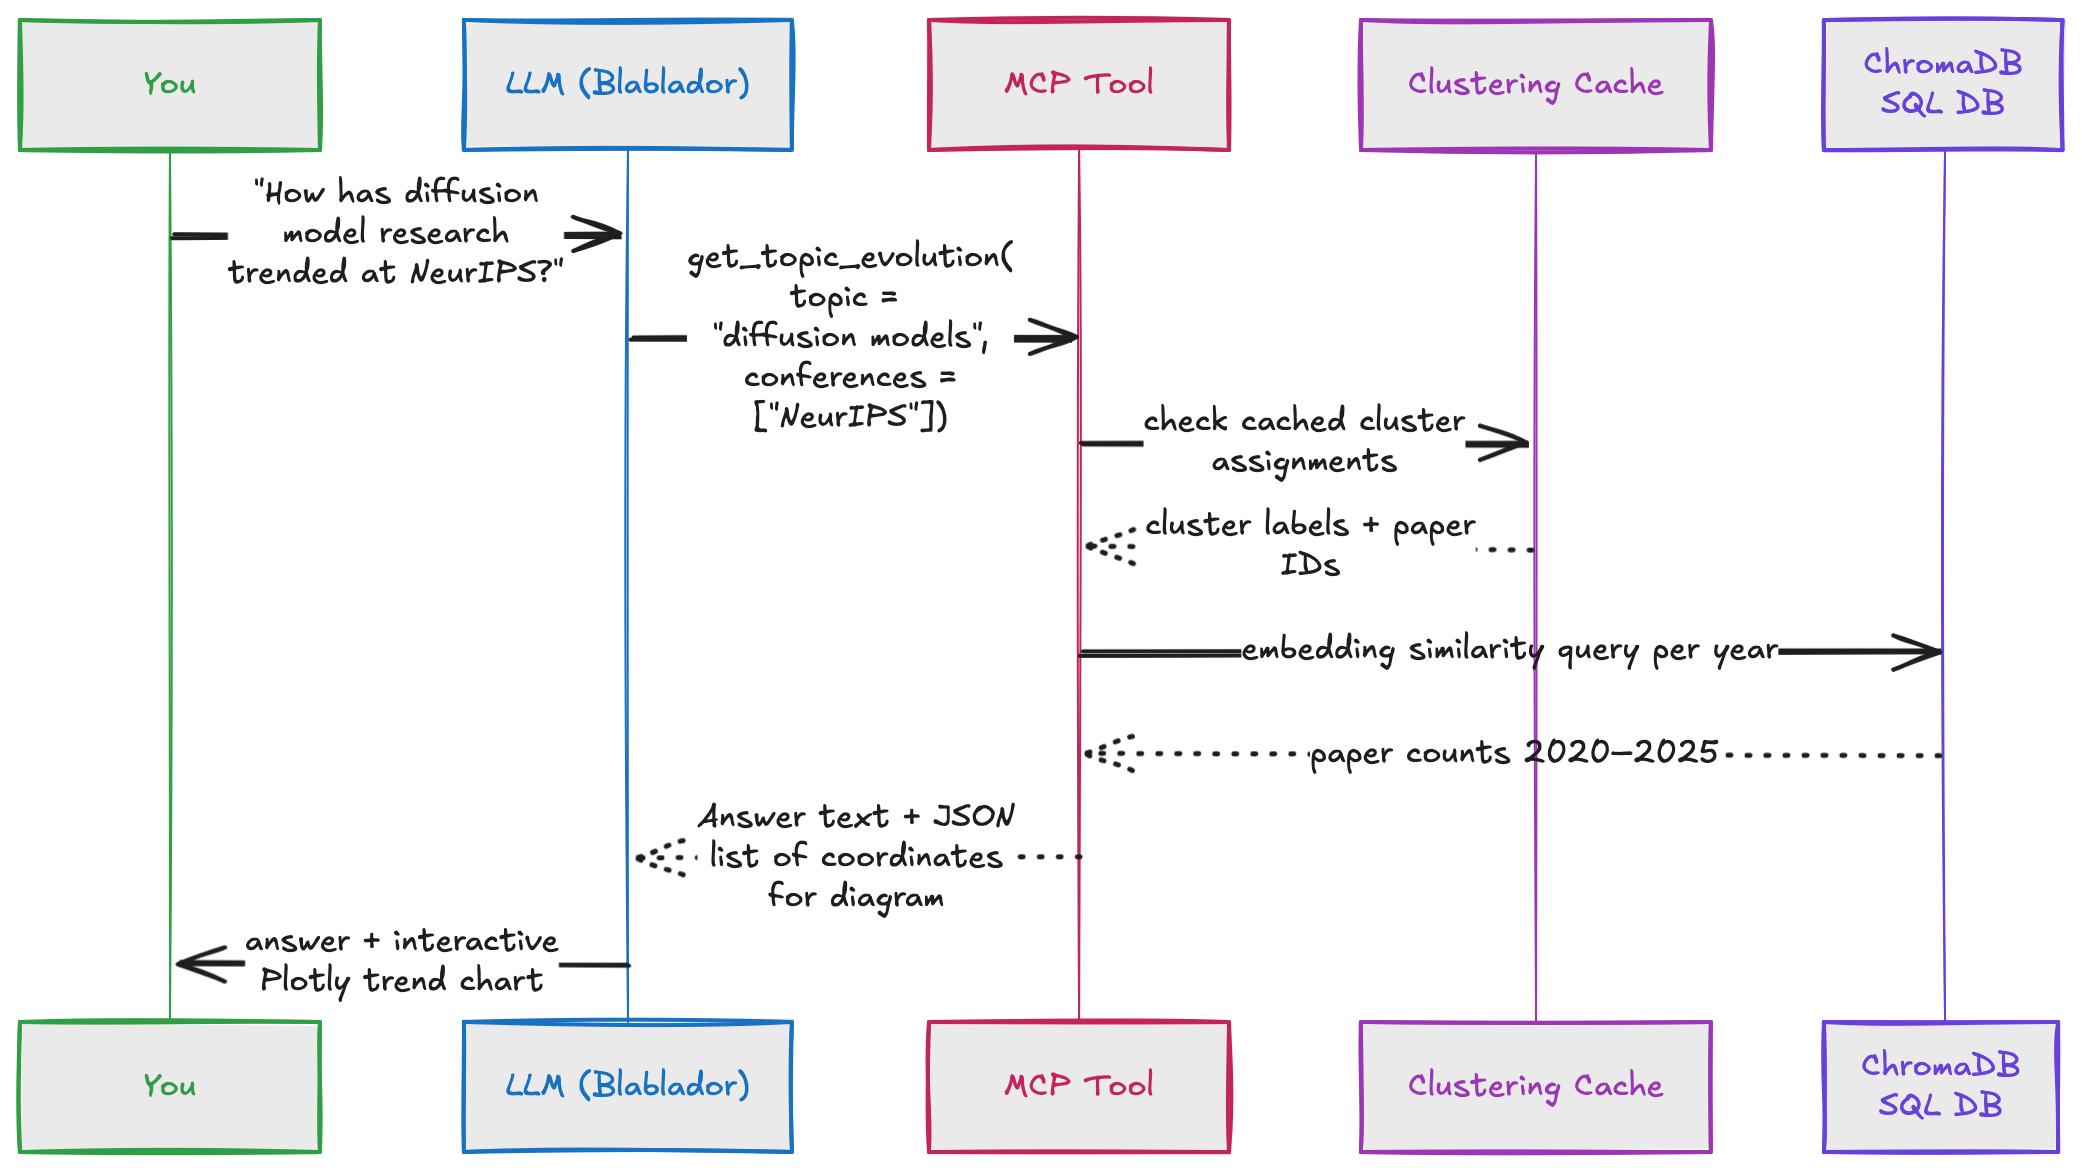
\includegraphics[width=0.9\textwidth]{images/Agentic-Loop-Diagram.png}
  \end{center}
\end{frame}

% 10 — WHY "AGENTIC"?
\begin{frame}{This Is Genuine Agency}
  \small
  \begin{tabularx}{\textwidth}{lX}
    \toprule
    \textbf{Property}             & \textbf{How Abstracts Explorer satisfies it}                                                     \\
    \midrule
    \textbf{Goal-directed}        & Answers open-ended research questions, not just keyword lookups                                  \\
    \textbf{Tool use}             & LLM autonomously selects among 6 specialised tools                                               \\
    \textbf{Multi-step reasoning} & Query rewriting $\rightarrow$ retrieval $\rightarrow$ optional tool loop $\rightarrow$ synthesis \\
    \textbf{Grounded}             & Every answer cites the source abstracts                                                          \\
    \textbf{Persistent state}     & Conversation history, tool results                                                               \\
    \textbf{Human in the loop}    & Follow-up questions and feedback                                                                 \\
    \bottomrule
  \end{tabularx}
\end{frame}

\begin{frame}{Working Today for 8 Conferences}
  \textbf{Today}
  \begin{itemize}
    \item 8 conferences, multi-year data (NeurIPS $\cdot$ ICLR $\cdot$ ICML $\cdot$ CHI $\cdot$ HAICON $\cdot$ \ldots)
          \begin{itemize}
            \item Plugin system makes it easy to add more - use the issue template on Github to request your favourite conference!
          \end{itemize}
    \item 6 MCP tools, automatic RAG integration
    \item Conference data registry: share conference data across installations
    \item $>$ 90\% Python test coverage $\cdot$ Docker deployment
  \end{itemize}
  \vspace{0.5em}
  \textbf{Planned}
  \begin{itemize}
    \item More agentic behaviours: build personalised schedule based on user prompt, existing ratings, and conference data
  \end{itemize}
\end{frame}

% 11 — DEPLOYMENT
\begin{frame}[fragile]{Easily Deployed with Podman Quadlets}
  Quadlets are \texttt{systemd} unit files that describe containers --- Podman generates real \texttt{.service} units from them automatically.\\[0.5em]

  \begin{block}{Single command to install}
    curl -fsSL https://raw.githubusercontent.com/thawn/abstracts-explorer/main/scripts/install-quadlets.sh | bash
  \end{block}

  \textbf{Advantages:}
  \begin{itemize}
    \item Secure: almost everything runs in user space --- root permissions needed only for ports 80 and 443
    \item Systemd-native service management
  \end{itemize}
  \vspace{0.3em}
  \textbf{Prerequisites:} Podman installed, \texttt{podman generate systemd} in your PATH, curl installed.\\[0.3em]
\end{frame}

\begin{frame}{Mini Hackathon}
  \Large
  \begin{tabularx}{\textwidth}{lX}
    \parbox[c]{5em}{\centering
\includegraphics[width=5em]{images/abstracts.hzdr.de.png}} & \parbox[c]{\linewidth}{\textbf{Try it out!} $\rightarrow$ \url{https://abstracts.hzdr.de/}}                                                                                                                                                                                            \\
    \parbox[c]{5em}{\centering
\includegraphics[width=5em]{images/github.png}}            & \parbox[c]{\linewidth}{\textbf{Contribute on Github} $\rightarrow$ \url{https://github.com/thawn/abstracts-explorer}}                                                                                                                                                                  \\
    \parbox[c]{5em}{\centering
\includegraphics[width=5em]{images/first-issue.png}}       & \parbox[c]{\linewidth}{\raggedright\textbf{Check out good first issues} $\rightarrow$ {\large\href{https://github.com/thawn/abstracts-explorer/issues?q=is\%3Aissue\%20state\%3Aopen\%20label\%3A\%22good\%20first\%20issue\%22}{https://github.com/thawn/abstracts-explorer/issues}}}
  \end{tabularx}
\end{frame}

% 13 — TAKE-AWAY
\begin{frame}{Summary}

  Abstracts Explorer is a small but complete example of Agentic AI for science:
  \begin{itemize}
    \item Domain-specific knowledge base (conference abstracts)
    \item Local-first, privacy-respecting (runs on your laptop or institute server)
    \item Open tool protocol (MCP) --- swap the LLM backend without rewriting the tools
    \item Human-in-the-loop design --- ratings, export, and curation stay with you
  \end{itemize}
  \vspace{0.3em}
  \textbf{Come talk to me at the poster!}\\
  Try the demo $\rightarrow$ \url{https://abstracts.hzdr.de/} $\rightarrow$ don't forget to donate your data\\
  Contribute on Github \faGithub~\url{https://github.com/thawn/abstracts-explorer}
\end{frame}

\begin{frame}{Thank You!}
  \begin{center}
    \Large
    \textbf{Questions?}
  \end{center}
\end{frame}

% BACKUP SLIDES
\appendix

% 9 — ARCHITECTURE
\begin{frame}{Architecture}
  \begin{center}
    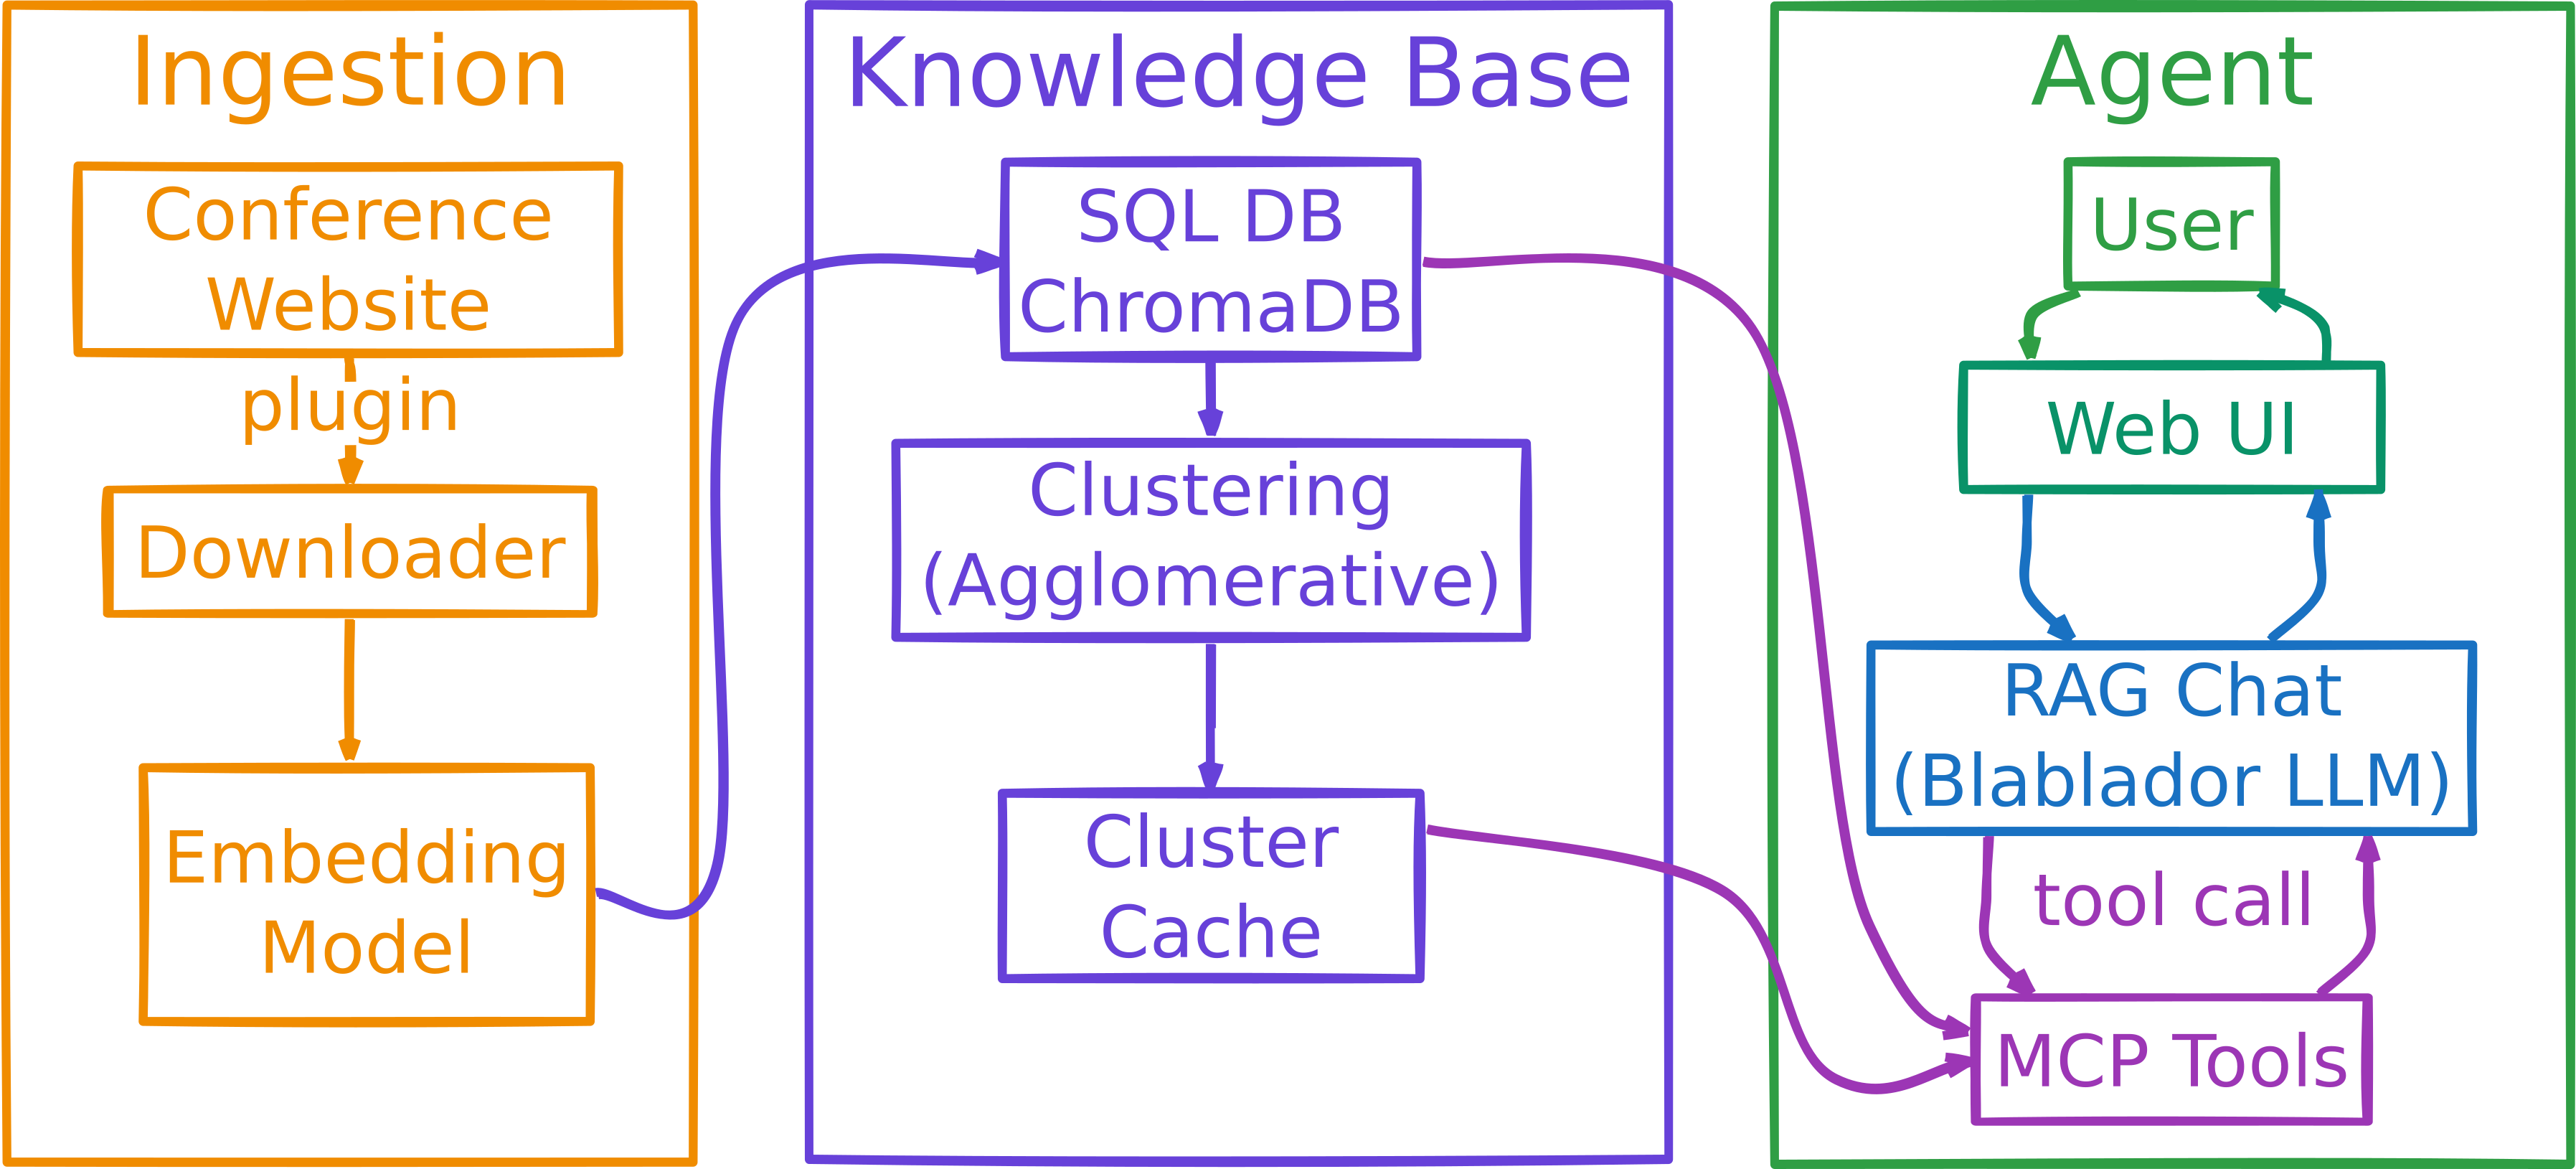
\includegraphics[width=\textwidth]{images/architecture.png}
  \end{center}
\end{frame}

\end{document}
